\chapter{Theory}
\label{sec:grundlagen}

\section{Econometric Motivation}
\subsection{Portfolio Theory}
When trying to calculate the optimal portfolio, to maximize returns while still minimizing risk, or in explaining effects of risk diversification, the need for a portfolio theory arises. This theory should explain how inverstors make sensible decisions in the optimisation problem of risk versus return, as well as explain how diversification in experiment achieves such a feature. While previous studies \cite{Markowitz_1952} of the models have shown that lesser correlations result in risk reduction, the effect can be used efficiently to more accurately predict stock returns in the future. The model proposed by Markowitz can achieve risk-minimisation, while still providing return maximisation. The goal of the model is to create action instructions enabling investors to build their optimal portfolio based on the combination of investment opportunities. To achieve this, the theory is based upon a set of assumptions.
\begin{itemize}%Markowitz Assumptions
	\item The investor is an agent only interested in amassing its own wealth. It is only interested in basing decisions on known financial information. 
	\item The investor agent acts only rational and usage-maximizing, weighing only profits against risks.
	\item Risks should always be averted, so high-risk actions should only be taken if the expected return grows disporportionately higher. 
	\item The capital market is complete. 
	\item Systematic risk affects all assets, while specific risk only affects the respective specific assets. 
\end{itemize}
If the above assumptions hold, an investor will always choose a portfolio over another, if the expected return $\mu$ is greater or equal, with a smaller variance $\sigma$, or if the return $\mu$ is greater while the variance $\sigma$ is equal. A complete capital market is a market with negligible transaction costs and perfect information, and the existence of a price for every asset in every possible state of the world \cite{Buckle_2018}. Due to the inequalities in these conditions, only unique portfolios will appear in the theory. A solution to the equations is called an efficient portfolio. Efficient portfolios avert unreasonably high overall risks while retaining a relatively high expected return.  \newline
When obtaining an asset with money $x_0$ and selling it at a later date for money $x_1$, the ratio between the two can be defined as the absolute return $R$. 
\begin{equation}%Return simple definition
	R = \frac{x_1}{x_0}
\label{eq: Return simple definition}
\end{equation}
From this, we can easily derive the rate of return, or relative return, which will in later chapters will be regarded as \textit{return} $r$. 
\begin{equation}%Return Rate Definition
	r = R-1 = \frac{x_1 - x_0}{x_0}
\label{eq:Return_Rate_Definition}
\end{equation} 
These definitions hold for buy-sell actions, as well as short selling, where the investor first sells assets from the broker and then rebuys them at a later date, resulting in a sell-buy action. In the case of short selling, double negative signs in the fractions arise, but cancel out. Risks are, for now, expected to always be real positive values, never exactly zero. This leads to a normalized system of investments through weights $w_i$ describing how much of the total monetary aggregate is invested into asset or portfolio $i$
\begin{equation}%Normalization of Sum of Investments
	\sum_{i=1}^{n} w_i x_0 = x_0.
\label{eq: Normalization of Sum of Investments}
\end{equation}
The rate of return of the total investment is
\begin{equation}%total rate of return
	r = R-1 = \sum_{i=1}^{n} R_i w_i - \sum_{i=1}^{n} w_i = \sum_{i=1}^{n} r_i w_i.
\label{eq: total rate of return}
\end{equation}
The Markowitz Mean-Variance Portfolio Theory then models the rate of returns on assets as random variables. A global optimisaition is then applied to find the best weights for each part of the portfolio. The volatility of an asset is surrogated through the proportional variance. We find the Markowitz problem to be the optimisation of
\begin{subequations}
	\label{eq:Markowitz Optimisation Problem}
	\begin{align}
	\text{\textbf{min}} \Bigg( 0.5 \bm{w}^{\top} \Sigma \bm{w} \Bigg)         \label{eq:Optimisation} \\
	\text{subject to }\bm{m}^{\top} \bm{w} \geq \mu_b \text{ and }\bm{e}^{\top}\bm{w}=1         \label{eq:Conditions}
	\end{align}
\end{subequations}
Where $w$ is the vector of weights, $\Sigma$ the covariance matrix of the random random vector $z$ containing the returns, $m^{\top}w$ the mean of the random variable, $w^{\top} \Sigma w $ is the variance and $\mu_b = \mathbb{E}[r_b]$ the acceptable baseline expected return. Also, $e$ is the unit vector of the arbitrary dimension suiting the problem and $n$, the number of possible assets. To solve this nonlinear problem, Karush-Kuhn-Tucker (KKT) conditions \cite{Kuhn_Tucker_2014} can be formulated, which allow the analytic and algorithmic solution of the problem. At first, showing that the problem is feasible guarantees the existence of a finite optimal value, as well as the existence of a solution to find the optimal value. If the acceptable baseline expected return is below the mean, $\mu_b > \bm{m}^{\top}\bm{w}$, the obtained solution is a least variance solution. The mean return associated with the least-variance solution $\mu_{lv}$ is
\begin{equation}%mean return least-variance solution
	\mu_{lv} = \frac{\bm{m}^{\top} \Sigma^{-1}\bm{e}}{\bm{e}^{\top} \Sigma^{-1}\bm{e}}
\label{eq: mean return least-variance solution}
\end{equation}
The case $\mu_b = \bm{m}^{\top}\bm{w}$ is also possible, where we can identify that the optimal portfolio usually is two-fold. 
\begin{equation}%optimal distribution of weights
	w = (1-\alpha) \frac{\Sigma^{-1}\bm{e}}{\bm{e}^{\top}\Sigma^{-1}\bm{e}} + \alpha \frac{\Sigma^{-1}\bm{m}}{\bm{e}^{\top}\Sigma^{-1}\bm{m}} = (1-\alpha)w_{lv} + \alpha w_{mk}
\label{eq: optimal distribution of weights}
\end{equation}
Any solution to the Markowitz problem can be presented as a linear combination of these two sets of weights: the risk-free least-variance solution, and the market portfolio, which incorporates the rest of the knowledge about the market. The previous statement is also known as the \textit{Two Fund Theorem}. We can obtain the solution space by finding all possible curves parametrised by 
\begin{subequations}%Solution space curves
	\label{eq:Solution space curves}
	\begin{align}
	\Big( \sqrt{\bm{w}_i^{\top}}, r_i \Big) = \Big( \sqrt{var(r_i)}, \mathbb{E}(r_i) \Big)        \label{eq:Solution space curve} \\
	\text{where } r_i = \bm{w}_i^{\top}r, \text{ as } i \text{, the number of assets, varies from } 0 \text{ to } +\infty         \label{eq:Solution space curve conditions}
	\end{align}
\end{subequations}
If a risk-free asset is introduced now, as is a good approximation for very low risk securities, e.g. treasury bonds, some properties of the described system change. First, the \textit{One Fund Theorem} is introduced. It states, that for the case of available risk-free assets, the least variance portfolio is always comprised of only those risk-free assets. Also, every efficient portfolio can be created using a combination of these risk-free portfolios and another Fund $F$ with risk $>0$. This leads directly towards the Capital Asset Pricing Model (CAPM), which provides and solves for optimal portfolios, assuming risk-free assets exist. \newline 
This still leaves open the question of how to optimally calculate a covariance matrix, so that it is the closest approximation of the true covariance matrix. A simple theory of construction is given by the sample covariance matrix, 
\begin{equation}
	K = \frac{1}{D} (\bm{r}-\bm{\hat{\mu}})(\bm{r}-\bm{\hat{\mu}})^{\top}.
	\label{eq:sample_cov}
\end{equation}
Where $\bm{\hat{\mu}}$ is again the mean of the asset samples respectively. If the number of days of observation $D$ is large enough, this estimation is called the maximum likelihood estimator. It provides an unbiased estimation, but in practice, especially if the ratio $N/D$ is not small, the matrices often become unstable or singular. Other methods include the Ledoit-Wolf estimation, where shrinkage is used to estimate the covariance matrix \cite{Ledoit_2004}, or Gaussian Processes, which will be discussed in sections \ref{sec:GPLVM} and \ref{sec:gplvm_finance}. 
\label{sec:portfolio}
\cleardoubleoddpage

\subsection{Capital Asset Pricing Model}
Within the Capital Asset Pricing Model (CAPM), a linear model including latent spaces, we can define the market portfolio $r_M$ as
\begin{equation}%market portfolio capm
	r_M = \begin{bmatrix} r_f \\ r \end{bmatrix}^{\top} \begin{bmatrix} 1-\bm{e}^{\top} \Sigma^{-1}(\bm{m}-r_f\bm{e}) \\ \Sigma^{-1}(\bm{m}-r_f\bm{e}) \end{bmatrix},
\label{eq: market portfolio capm}
\end{equation}
which leads to the expected return on any asset in CAPM
\begin{equation}%expected return any asset capm
	\mu_i = r_f \beta_i(\mu_M -r_f) \text{,}
\label{eq: expected return any asset capm}
\end{equation}
where $\beta_i$ is the covariance relation of market portolio $r_M$ and individual asset $i$. $\beta$ is understood to be the risk, 
\begin{equation}%beta capm
	\beta_i = \frac{\sigma_{iM}}{\sigma_M^2}.
\label{eq: beta capm}
\end{equation}
Then, the expected return of the portfolio $\mu_r$ satisfies 
\begin{equation}%expected return portfolio
	\mu_r = r_f + \frac{\mu_M - r_f}{\sigma_M}\sigma_r,
\label{eq: expected return of portfolio capm}
\end{equation}
where for a given portfolio $r$ the mean portfolio return $\mu_r = \mathbb{E}(r)$ and $\sigma_r^2 = \text{var}(r)$. The line of efficiency is then given by 
\begin{subequations}%efficiency line capm
	\label{eq:efficiency line capm}
	\begin{align}
	\mu_M = \mathbb{E}(r_M) = r_f + (\bm{m}-r_f\bm{e})^{\top}\Sigma^{-1}(\bm{m}-r_f\bm{e}),         \label{eq:Expected value market} \\
	\sigma_M^2 = \text{var}(r_M) = (\bm{m}-r_f\bm{e})^{\top}\Sigma^{-1}(\bm{m}-r_f\bm{e}).         \label{eq:variance market}
	\end{align}
\end{subequations}
Recalling the relation \ref{eq:Return_Rate_Definition}, where the return rate was defined, we can find the CAPM pricing formula, substituting the sell-price $x_1$ with $P$, and the buy-price $x_0$ with $Q$. 
\begin{equation}%capm pricing formula
	P = \frac{\mu_Q}{1+r_f+\beta_r(\mu_M-r_f)}
\label{eq: capm pricing formula}
\end{equation}
The main connection between the expected value of the return of an asset and its risk is described by
\begin{equation}%expected return with risk capm
	\mathbb{E}[\bm{r}_n] = \bm{r}_{rf} + \beta_n\mathbb{E}[\bm{r}_{m} - \bm{r}_{rf}] = \bm{r}_f + \beta_n\mathbb{E}[\bm{r}_{me}]. 
\label{eq:expected_return_with_risk_capm}
\end{equation}
with the risk-free ($\beta=0$) return rate $\bm{r}_{rf}$, which is the expected return rate for a zero-risk portfolio. For any portfolio with risk $\beta_n \neq 0$, the excess return of the market $\bm{r}_{me} = \bm{r}_m - \bm{r}_f$ applies, and the investor is compensated with a higher expected return. Note, that all $\bm{r}_{f/m/me} \in \mathbb{R}^D$ for $D$ different days. So equation \ref{eq:expected_return_with_risk_capm} can be rewritten in terms of the excess return $\bm{r}_e = \bm{r} - \bm{r}_f$ with excess return of an asset n: $\bm{r}_{e,n}$,
\begin{equation}%excess return
	\mathbb{E}[\bm{r}_{e,n}] = \beta_n\mathbb{E}[\bm{r}_{me}].
\label{eq: excess return}
\end{equation}


\subsection{Arbitrage Pricing Theory}
\label{sec:apt}
If the model is then expanded to include multiple additional risk factors $\bm{F}$, other than systematic risk factors of the market and specific risk factors of the assets, we arrive at Arbitrage Pricing Theory (APT) \cite{Ross_2013}.
APT assumes, that every asset return follows a factor structure with an additional noise term $\epsilon_n$, that is modeled as a Gaussian with zero mean and variance $\sigma_n^2$ \cite{Ross_n_Roll_1995}. The factor structure allows the Arbitrage pricing theory to incorporate other factors, which different studies have shown to be at least partly influential on the predictive power of CAPM. One of the aforementioned models is the Fama-French three factor model, consisting of the expected returns, the difference between returns in portfolios of small and big stocks, and the returns of portfolios containing high and low stocks \cite{Fama_1993} \cite{Fama_1996}.
\begin{equation}%three factor model
	\mathbb{E}[\bm{r}_{M}] - \bm{r}_{f} = \bm{\beta}_{M}[{E}[\bm{r}_{M}] - \bm{r}_{f}] + \bm{\beta}_{SMB}[\mathbb{E}[R_{SMB}]] + \bm{\beta}_{HML}[\mathbb{E}[R_{HML}]].
\label{eq: Three factor model}
\end{equation}
The expected returns are shown to behave like 
\begin{subequations}%Arbitrage Pricing Model, asset return structure and expected return excess.
	\label{eq:Arbitrage Pricing Model}
	\begin{align}
	\bm{r}_n = \alpha_n + \bm{F}\bm{\beta}_n + \epsilon_n         \label{eq:asset return factor structure} \\
	\mathbb{E}[\bm{r}_{e,n}] = \mathbb{E}[\bm{F}]\bm{\beta}_n         \label{eq:expected excess returns}
	\end{align}
\end{subequations} 
This equation for the asset return factor structure $\bm{r}_{n}$ can then be rewritten, so that it matches the form of a Gaussian Process Latent Variable Model, which will be explained in detail in section \ref{sec:GPLVM}. 
\begin{equation}%GPLVM form of Arbitrage Pricing Theory
	\bm{r}_{n,:} = f(\bm{B}_{n,:}) + \epsilon_n
\label{eq: GPLVM form of Arbitrage Pricing Theory}
\end{equation}
where $:$ stands for all entries in the specified dimension, and $\bm{B}$ is the factor matrix constructed from the $\bm{\beta}_n$. The three factor model also has shortcomings \cite{Fama_French_2004}, which especially arise from the momentum effect, where due to inverstors beliefs in well performing stocks over a timespan of e.g. 3-12 months, these stocks continue to do well afterwards. The same effect also applies to stocks that do not do well over such a timespan, they will probably not do well for the next few months after. \newline
In APT, the factors are unobserved quantities, that can be inferred using e.g. PCA. The drawback of PCA, assuming an error with fixed variance for each element of the return matrix $r$, highlights that alternatives are needed. Another approach was factor analysis \cite{Everitt_1984}, which allowed different noise variances for each asset contained in $r$. Since there is no analytic result to the optimization of the marginal distribution in this case, these can be solved iteratively using the expectation maximization algorithm \cite{Bishop_2006}. 

\label{sec:capm}
\cleardoubleoddpage

\subsection{ARCH and GARCH}
\subsubsection{ARCH}
An econometrics model for time series data describing the variance of the current error through statistics is the autoregressive conditional heteroskedasticity (\textit{ARCH(q)}) model (xxx). The ARCH model is based upon the assumption, that the current error term is a function of the previous time periods error terms. In terms of variance, often the square of the previous time steps error terms are used. In practice, the ARCH model is often used for modeling financial time series exhibiting time-dependent volatility, or so called volatility clustering, e.g. periods of higher volatility, followed by periods of comparably lower volatility, and the other way around. The model is specified through the time series terms.
\begin{equation}
	\epsilon_t = \sigma_t z_t
\label{eq: ARCH process}
\end{equation}
Here, $\epsilon_t$ denotes the error terms that make up the ARCH process, $z_t$ is a random variable defined by a strong white noise process, and the series $\sigma_t^2$ is educed as 
\begin{equation}
	\sigma_t^2 = \alpha_0 + \sum_{i=1}^{q}\alpha_i \epsilon_{t-i}^2,
\label{eq: ARCH sigma series}
\end{equation}
where all free parameters $\alpha_0, \alpha_i > 0$. The ARCH(q) model was shortly after refined as GARCH(p,q) model, where an important generalization was implemented into the model. 

\subsubsection{GARCH}
The Generalized autoregressive conditional heteroskedasticity (\textit{GARCH(p,q)}) model is the generalization of the ARCH(q) model, which directly includes lag. It is defined by 
\begin{subequations}
	\label{eq:GARCH definition}
	\begin{align}
	y_t = X-t'b + \epsilon_t,         \label{eq:GARCH main process} \\
	\epsilon_t | \psi_{t-1} ~ \mathcal{N}(0,\sigma_t^2),         \label{eq:GARCH noise} \\
	\sigma_t^2 = \omega + \sum_{i=1}^{q}\alpha_i \epsilon_{t-i}^2 + \sum_{i=1}^{p}\beta_i \sigma_{t-i}^2.         \label{eq:GARCH variance} 
	\end{align}
\end{subequations}
We then find the lag length through estimating the optimal ARCH process and estimating autocorrelations. 
\begin{subequations}
	\label{eq:GARCH lag length}
	\begin{align}
	y_t = a_0 + \sum_{i=1}^{q}a_i y_{t-i} + \epsilon_t,         \label{eq:GARCH lag ARCH} \\
	\rho = \frac{\sum_{t=i+1}^{T}(\hat{\epsilon}_t^2 -\hat{\sigma}_t^2)(\hat{\epsilon}_{t-1}^2 -\hat{\sigma}_{t-1}^2)}{\sum_{t=1}^{T}(\hat{\epsilon}_t^2 -\hat{\sigma}_t^2)},         \label{eq:GARCH estimate autocorrelations}
	\end{align}
\end{subequations}
For large samples, GARCH errors are implicated if the standard deviation $\rho(i)=1/\sqrt{T}$. Based on this, the Ljung-Box test can be applied to base a decision if to reject or accept it´s null hypothesis, that there are no ARCH or GARCH errors. In later chapters of this work, the GARCH process is sampled using a Hamilton Chain Monte Carlo algorithm (xxx pyflux), and then used to create datasets that are normed on the expected volatility. 
\label{sec:arch}
\cleardoubleoddpage


\section{Stochastic Process Models}
\subsection{Introduction}
Assessing the chance of something happening in real life, one encounters more than just probabilities. It is directly connected to the model of our world, the probabilities of certain events happening inside the model, and how good the model actually resembles what we understand to be the truth. Models can be created using two trains of thought (xxx schools?) in statistics, about how to assign probabilities from observing events. Firstly, there is frequentist statistics, centered around the idea, that there is a fixed probability for an event that can, in theory, be derived from axioms[xxx]. Observing an event many times shall then directly converge towards the true value. Observe a coinflip as an example, the difference can be illustrated quite easily. If the coin is flipped often enough and the coin is fair, then we observe that every time the coin is flipped, the probabilities for observing "\textit{heads}" and "\textit{tails}" will converge another step towards $0.5$. 
\begin{figure}[h!]%Cloinflip
	\centering
	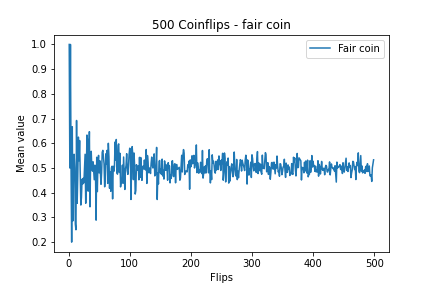
\includegraphics[width=4in]{img/05_1/fair_coinflip.png}
	\caption[Fair Coinflip]
	{A simulated fair coin flip, with 500 iterations of either \textit{heads} (1) or \textit{tails} (0). }
\end{figure}
If we repeat the experiment with an unfair coin instead, our assumption of a fair coin will now still lead us to assume the probabilities for \textit{heads} and \textit{tails} were $0.5$, just like in a perfect system. Here we are still assuming that if we observe enough events, the probabilities should be verified by the experiment. Statistical uncertainty in observing a fair coin could shift the observed probabilities for a while, but will always converge. Only after observing many events, we would start to question the assumptions we had at the beginning, e.g. of the coin being fair, because convergence is slow. 
\begin{figure}[h!]%Coinflip Comparison fair and unfair coin
	\centering
	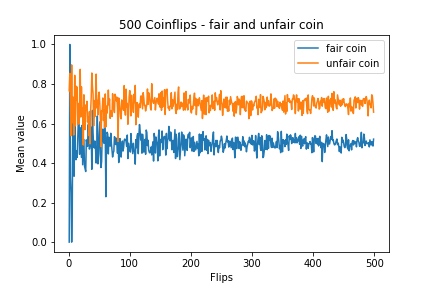
\includegraphics[width=4in]{img/05_1/unfair_coinflip.png}
	\caption[Fair and unfair coinflip comparison]
	{A simulated fair coin flip (blue) compared to the unfair coin flip (orange). Even though both tend towards different values for large sample sizes, in the first few flips, it is very hard to distinguish which coin is fair. Experimental conditions are the same as with the simulated fair coin flip.}
\end{figure}
So, from the frequentists perspective, if we were in the situation of playing coinflip with an unkown coin, it would take a long time, until we would accept the possibility that our model could be wrong. This inherent trust into the models is therefore used mostly in fields like physics, where the theory is assumed to reflect the ground truth no matter what, with the assumption that constants are always constant and the set of rules never changes, independent of where you are in the universe. This is called the Noether theorem, but since it only applies to the set of rules in physics, where controlling variables can be enforced with great precision, other fields need a more flexible theory to determine the probability of an event. So, assuming there are variables influencing our system in ways we cannot foresee with absolute precision, we need to be able to update the expected probabilities as a function of our observations. Since the probabilities are a crucial part of the model we applied to reality in the first place, we need to find a model that can be updated each time an observation took place. Bayesian statistics allows us to update our beliefs along the way. It dates back to Thomas Bayes, who in his essay "\textit{An essay towards solving a problem in the doctrine of chances}" [xxx] introduced the first version of this idea. Our percieved reality can always be flawed, not limited to a fair or unfair coin, but models for reality of all sorts can have intrinsic flaws, that can be quantified using this method of determining probabilities and updating models, along the way. Through this, probabilities become dependent on believability and credibility, confidence in decisions or environmental variables of the problem. Creating a model in bayesian statistics also allows for a causal bias introduced into the model, before observations even took place. So, if for example you would consider playing against someone with a coin you do not yet know to be fair, it is best to assume the coin is unfair at first. Noticing that a coin is unfair faster, and with higher probability, to update the model is valuable information. Previously we noticed, that the flexibility of bayesian models allow us to take into account environmental variables, but how many of those will actually lead to better predictions from the model? Occams Razor (xxx) is a good rule to follow, which would roughly translate to "\textit{choose a model as complicated as necessary but no more than that}". Or, in other words, a more complex model with more hyperparameters will in the end lead to better explanation ("a better fit") of the observed data, but prediction power will intrinsically decrease along the way, due to more noise being learned as a feature. 
\label{sec:introduction}
\cleardoubleoddpage

\subsection{Bayesian Statistics}
Models using the bayesian framework of statistics rely on conditional probability. These probabilities are conditioned on previous assumptions about the general environment. This can be surroundings, game states, environmental variables, etc. Since the properties of complex systems are majorly influenced by these traits, incorporating them into the model is of utmost importance. The general case of Bayes rule combines prior knowledge of the model, called a prior probability, with the observed evidence and its likelihood to form the posterior probability. The posterior probability can be interpreted as the probability of observing a certain set of observations dependent on the likelihood of the observations, given the model. 
\begin{equation}%Bayes Rule
	P(A|B) = \frac{P(B|A) P(A)}{P(B)}
\label{Bayes Rule for probabilities. }
\end{equation}
Here, A is the proposition and B the evidence, and we try to get the posterior $P(A|B)$, the degree of belief in $A$ if we have accounted $B$ to be true. $P(A)$ is the prior, the initial belief in $A$, while $P(B)$ is the likelihood of the evidence being true. This rule currently applies only to probabilities, but it can just as well be scaled up to probability distributions.
\begin{equation}%Bayes rule distributions
	p(A|B) = \frac{p(B|A) p(A)}{p(B)}
\label{Bayes Rule for probability distributions. }
\end{equation}
Probability distributions, which are factors defining models, can be tested for reliability via Bayes rule too. Also using Bayes rule, we can test our model assumptions and compare models. 
\begin{equation}%Bayes Rule Models and Data
	p(M|D,I) = \frac{p(D|M,I) p(M|I)}{p(D|I)}
\label{Bayes Rule for Model Comparison}
\end{equation}
Here, $M$ is the model in question, while $D$ is the observed Data, and $I$ is the previously known information of the system. We can then formulate a hierarchical Bayesian workflow.
\begin{enumerate}%Bayesian Workflow
	\item Use Bayes Rule to construct a naive model using only prior knowledge
	\item Update knowledge inside naive model 
	\item Create more complex model using Bayes rule for models
	\item Update knowledge about complex model
	\item repeat steps 1-4 until KL-Divergence converges to 0.
\end{enumerate}
%When we maximize the likelihood trough the Maximum Likelihood Method, we can approximate the true parameters through the model parameters. [xxx]
Every bit of knowledge we have about the system is now encoded in probability distributions, but to calculate this workflow, we need some class of probability distributions, that is sensible to use in most models, and which can preferrably be solved analytically. In experiments, we will see that this workflow is not as easy as expected, since the evidence is often intractable (xxx look up from VB Wikipedia), which then can only be evaluated approximately. Also, we need to take into account, that the total solution space of Bayesian priors may not contain the solution we try to achieve, because the true model may be something very different, from what we originally thought it was. Here Occams Razor is again the doctrine we use to make decisions about model choice: Our model shall be complicated enough to grasp the underlying dynamic, but needs to be naive enough to not learn noise as a feature. This leads to Gaussian processes, since they have a lot of convenient properties. The priors of Gaussian Processes ($\mathcal{GP}$) are appropriate and have infinite basis functions. These are flexible enough for nonlinear models, but still retain analytic solutions. Through this, they are especially computationally feasible. Also, Student-\textit{t}-processes, as they are scaled Gaussian processes, seem to be a logical choice. Even though they are more restrained in the amount of computation tasks that can be done analytically, compared to the Gaussian Processes. 

%prior VB section
In applications of the Bayes rule there are posterior terms containing the information about the data, but sometimes they have combinatorially large search spaces. This leads to the intractability of these terms, represented by $\int_X P(Y,X)dX$.
\begin{equation}%Bayes with intractable term
	P(X|Y) = \frac{P(Y|X)P(X)}{P(Y)} = \frac{P(Y|X)P(X)}{\int_Z P(Y,X)dX}
	\label{eq:Bayes_with_intractable_term}
\end{equation}
To obtain the approximation using Variational Bayes, we introduce a variational distribution. 
\begin{equation}%Variational Distribution
	Q(X) \approx P(X|Y)
	\label{eq: Variational Distribution}
\end{equation}
This distribution $Q(X)$ is restricted to be of a family of simpler distributions than the true distribution, e.g. a posterior, $P(X|Y)$. The distribution family is selected with the intention of finding a $Q(X)$ similarly enough to $P(X|Y)$ so that $Q(X)$ can be used instead of $P(X|Y)$. We use KL-divergence to measure the dissimilarity of the distributions, but with a slight variation. Instead of using a KL-version $D_{KL}(p|q)$ that is applied in the expectation propagation algorithm, we use the reverse KL-divergence. 
\begin{equation}%Expectation maximisation KL-Divergence
	D_{KL}(Q|P) \triangleq \sum_{X} Q(X) \log \frac{Q(X)}{P(X|Y)}
	\label{eq: Expectation maximisation KL-Divergence}
\end{equation}
given, that
\begin{equation}%ELBO Intro
	P(X|Y) = \frac{P(Y,X)}{P(Y)},
	\label{eq: ELBO Intro}
\end{equation}
the KL Divergence here can be rewritten as
\begin{subequations}%new KL for ELBO
	\label{eq:new_KL_ELBO}
	\begin{align}
		D_{KL}(Q|P) = \sum_{X}Q(X) \Big[\log \frac{Q(X)}{P(X,Y)}+\log P(Y)\Big]  \\
		= \sum_{X}Q(X) [\log Q(X) - \log P(X,Y)] + \sum_{X}Q(X)[\log P(Y)]. 
	\end{align}
\end{subequations}
After seeing that $P(Y)$ is constant with respect to $X$ and $\sum_{X}Q(X)=1$ because $Q(X)$ is a distribution, and rewritten with the definition of the expected value for a discrete random variable, we arrive at
\begin{equation}%evidence log
	\log P(Y) = D_{KL}(Q|P) - \mathbb{E}_X[\log Q(Y) - \log P(X,Y)] = D_{KL}(Q|P) + \mathcal{L}(Q)
	\label{eq:evidence_log}
\end{equation} 
Since $P(Y)$ is fixed under $Q$, maximizing $\mathcal{L}(Q)$ minimizes the KL Divergence from Q to P. $\mathcal{L}(Q)$ is also known as the Evidence Lower Bound, which will be important to the evaluation of models later on. The variational distribution is usually assumed to factorize over some partition of the latent Variables $X$. 
\begin{equation}%Variational Distribution Factorisation
	Q(X) = \prod_{i=1}^{M} q_i(X_i)
	\label{eq: Variational Distribution Factorisation}
\end{equation}
Using Variational Calculus we find that the best distribution in a Bayesian workflow with Variational Bayes is
\begin{equation}%VB best Distribution
	q_j^* (X_j|Y) = \frac{\exp(\mathbb{E}_{i\neq j}[\ln p(X,Y)])}{\int \exp(\mathbb{E}_{i\neq j}[\ln p(X,Y)]) dZ_j},
	\label{eq: VB best Distribution}
\end{equation}
where $\mathbb{E}_{i\neq j}[\ln p(X,Y)]$ is the expectation value of the logarithm of the joint probability of data and latent variables not in the partition. Due to circular depencies between the parameters, the evaluation of these in a program offers to be solved iteratively. With this, due to the type of the distribution $Q(X)$, an analytical approximation for the posterior probability can be achieved, allowing the iterative calculation of parameters of the model. Variational Bayes can be used out of the box. Stan provides an implementation known as Automatic Differentiation Variational Inference (ADVI, Kucukelbir) that approximates the posterior with a Gaussian as the variational approximation. For more details, see section \ref{sec:stochastic_gradient_ascent}.
\label{sec:bayes}
\cleardoubleoddpage

\subsection{Gaussian Processes}
Supervised Learning Machine Learning can be divided into two classes of problems, regression and classification. Where in Classification the machine learning algorithm should decide between discrete class labels, the output of a regression algorithm is usually a continuous quantity. Due to the nature of the Gaussian Processes suiting regression problems, a focus is put on these, even though Gaussian Processes can also solve classification problems \cite{Rasmussen_06}. There are several ways of interpreting a Gaussian process, the function space view, and the weight-space view. In the weigth space view, the Gaussian Process is pictured as a process, with infinity many basis functions with corresponding weights. In the function space view, the gaussian process is a distribution over functions, and inference takes place in the function space defined by the process. The Gaussian process, as mentioned in section \ref{sec:capm} and \ref{sec:apt}, is mainly used to find the covariance matrices, that encode the covariance structure of the problem. 

\subsubsection{Weight Space View}
A simple Gaussian process will be derived here. Starting with a standard linear regression model with Gaussian noise
\begin{subequations}%Linear Regression Gaussian
	\label{eq:Linear Regression Model}
	\begin{align}
	f(x) = \bm{x}^\top \bm{w}         \label{eq: linear regression function} \\
	y = f(\bm{x}) + \epsilon         \label{eq: observed target value} \\
	\epsilon \thicksim \mathcal{N}(0, \sigma_{n}^{2})
	\end{align}
\end{subequations}
Here $\bm{x}$ is the input vector, $\bm{w}$ is the vector containing the weigths, $f$ is the function value and $y$ the observed target value. Also, $\epsilon$ is the independent noise, and it follows an independent, identically distributed Gaussian distribution with zero mean and variance $\sigma_{n}^{2}$. The likelihood, as probability density of observations given parameters factors over the cases of the training set. 
\begin{subequations}%Likelihood in Weight Space View
	\label{eq:Likelihood Weight Space View}
	\begin{align}
	p(\bm{y}|X,\bm{w}) = \prod_{i=1}^{n} p(y_i|\bm{x}_{i}, \bm{w}) =  \prod_{i=1}^{n} \frac{1}{\sqrt{2\pi}\sigma_{n}} \exp \Big( -\frac{(y_i -\bm{x}_{i}^{\top}\bm{w})^2}{2\sigma^2_n}\Big)      \label{eq:likelihood wieght space 1} \\
	= \frac{1}{(2\pi\sigma_n^2)^{n/2}} \exp \Big( -\frac{1}{2\sigma_n^2 }|\bm{y}-X^{\top}\bm{w}|^2 \Big) = \mathcal{N}(X^{\top}\bm{w}, \sigma_n^2 I)         \label{eq:likelihood weight space 2}.
	\end{align}
\end{subequations}
$X$ is all the data points from the input, and $|x|$ stands for the euclidian length of a vector $x$. Also, a prior must be specified, containing our beliefs about the parameters before observing the input. Therefore, we will distribute the weights using a zero mean Gaussian prior with covariance matrix $\Sigma_p$, 
\begin{equation}%Weights Distribution
	\bm{w} \thicksim \mathcal{N}(\bm{0}, \Sigma_p).
\label{Distribution of weights using a zero mean Gaussian with covariance matrix.}
\end{equation}
To apply Bayes rule, we need a marginal likelihood, which acts as a normalizing constant, and is independent of the weights by integrating them out. 
\begin{equation}%marginal likelihood
	p(\bm{y}|X) = \int p(\bm{y}|X,\bm{w}) p(\bm{w}) d\bm{w}
\label{eq: Marginal likelihood as normalizing constant}
\end{equation}
The full Bayes rule in this case then becomes the following
\begin{equation}%Bayes Rule for Linear Regression
	p(\bm{w}|\bm{y},X) = \frac{p(\bm{y}|X,\bm{w})p(\bm{w})}{p(\bm{y}|X)}
\label{Bayes Rule for linear Regression}
\end{equation}
Using complete the square and ignoring the marginal likelihood, we find
\begin{equation}%unnormalized posterior
	p(\bm{w}|X,\bm{y}) \thicksim \mathcal{N}(\frac{1}{\sigma_n^2}(\frac{1}{\sigma_n^2}XX^{\top}+ \Sigma_p^{-1}), (\frac{1}{\sigma_n^2}XX^{\top}+ \Sigma_p^{-1})^{-1})
\label{Unnormalized posterior}
\end{equation}
With this, we can easily find the predictive distribution for $f_* \triangleq f(\bm{x}_*)$, by averaging the output of all possible linear models with respect to the Gaussian posterior,
\begin{subequations}%Gaussian posterior predictive distribution
	\label{eq:Gaussian posterior predictive distribution}
	\begin{align}
		p(f_*|\bm{x}_*,X,\bm{y}) = \int p(f_*|\bm{x}_*, \bm{w})p(\bm{w}|X,\bm{y}) d\bm{w}    \label{eq:predictive distribution 1} \\
		= \mathcal{N}(\frac{1}{\sigma_n^2}\bm{x}_*^{\top}(\frac{1}{\sigma_n^2}XX^{\top}+ \Sigma_p^{-1})^{-1}X\bm{y}, \bm{x}_*^{\top}(\frac{1}{\sigma_n^2}XX^{\top}+ \Sigma_p^{-1})^{-1}\bm{x}_*).         \label{eq: predicitve distribution 2}
	\end{align}
\end{subequations}
This model can easily be expanded by transforming the input into some high dimensional space using a set of basis functions and subsequently applying the linear model in this higher dimensional space. Applying the map $\phi(x) = (1,x,x^2,x^3,x^4,...)^{\top}$ would for example implement polynomial regression, during which a $D$-dimensional input vector $x$ is mapped into an $N$-dimensional feature space. This allows us to rewrite the model as
\begin{subequations}%Feature Space Gaussian process
	\label{eq:Feature Space Gaussian process}
	\begin{align}
	f(\bm{x}) = \phi(\bm{x})^{\top} \bm{w}         \label{eq: feature space model} \\
	f_*|\bm{x}_*,X,\bm{y}  \thicksim \mathcal{N}\Big( \frac{1}{\sigma_n^2}\phi(\bm{x}_*)^{\top}(\sigma_n^{-2}\Phi \Phi^{\top} + \Sigma_p^{-1})^{-1} \Phi \bm{y} , \label{eq: predictive distribution mean} \\
	 \phi(\bm{x}^{\top})(\sigma_n^{-2}\Phi \Phi^{\top} + \Sigma_p^{-1})^{-1} \phi(\bm{x}_*) \Big)        \label{eq: predictive distribution covariance} 
	\end{align}
\end{subequations}
where $\Phi(X)$ is the aggregation of all columns $\phi(\bm{x})$ for all cases in the data set in the transformed space. It presents a computational time benchmark when executing such a model, since the inversion of $N\times N$ matrices is of $\mathcal{O}(N^3)$ complexity. With high-dimensional feature spaces, reducing the argument of the complexity function is valuable. So, sometimes rewriting the equations as
\begin{equation}%rewritten Feature Space Gaussian Process evaluated in data space. 
	f_*|\bm{x}_*,X,\bm{y} \thicksim \mathcal{N}\Big( \phi_*^{\top}\Sigma_p\Phi(K+ \sigma_n^2 I)^{-1}\bm{y}, \phi_*^{\top} \Sigma_p \phi_* - \phi_*^{\top} \Sigma_p \phi_*(K+ \sigma_n^2 I)^{-1}\phi_*^{\top} \Sigma_p \phi_* \Big)
\label{Rewritten Feature Space Gaussian Process evaluated in data space.}
\end{equation}
is useful, since the complexity $\mathcal{O}(n^3)$ is the maximum complexity possible for $n$ datapoints \cite{Rasmussen_06}. Then, the kernel function $k(\bm{x},\bm{x'}) = k(\cdot , \cdot) = \phi_*^{\top} \Sigma_p \phi_*$ is easily identified. The kernel is often also called covariance function. \newline

\subsubsection{Function Space View}
This derivation can also be done in function space. Here, we can define a Gaussian Process as a collection of random variables, any finite number of which have a joint Gaussian distribution. Since a Gaussian process is solely defined by its mean and kernel function, it can be written as
\begin{subequations}%Gaussian process function space view
	\label{eq:Gaussian_process_function_space_view}
	\begin{align}
	m(x) =\mathbb{E}[f(x)]         \label{eq:function space view mean} \\
	k(\bm{x},\bm{x'}) = \mathbb{E}[(f(\bm{x})-m(\bm{x}))(f(\bm{x'})-m(\bm{x'})))]         \label{eq:function space view covariance function} \\
	f(x) \thicksim \mathcal{GP}(m(\bm{x}), k(\bm{x}, \bm{x'})).               \label{fuinction space view gaussian process}
	\end{align}
\end{subequations}
The Function space view notation will be the notation further on used in this thesis. Here, $\mathcal{GP}$ stands for a Gaussian Process, $m(\bm{x})$ is the mean function, and $k(\bm{x}, \bm{x'})$ is the kernel function. The consistency requirement, also marginalization property, states, that for a $\mathcal{N}$ $(y_a, y_b) \thicksim \mathcal{N}(\bm{\mu}, \Sigma)$ with general mean vector $\bm{\mu} = (m(\bm{x}_a), m(\bm{x}_b))^{\top}$ and covariance matrix $\Sigma$, the underlying $\mathcal{N}(y_a)$ is specified by $y_a \thicksim \mathcal{N}(\mu_a, \Sigma_{aa})$. $\Sigma_{aa}$ then is the submatrix of $\Sigma$ relevant to the distribution for $y_a$. Since the submatrixes are not intertwined in $\Sigma$, the examination of a larger set of variables does not change the distribution of a subset. Using the previously discussed linear regression model $f(x) = \phi(\bm{x})\bm{w}^{\top}$ with a gaussian prior on $\bm{w}$ we have mean and covariance
\begin{subequations}%Function space view linear regression mean and covariance
	\label{eq:Function space view linear regression mean and covariance}
	\begin{align}
	\mathbb{E}[f(\bm{x})] = \phi(\bm{x})^{\top} \mathbb{E}[\bm{w}] = 0         \label{eq:function space linear mean} \\
	\mathbb{E}[f(\bm{x})f(\bm{x'})] = \phi(\bm{x})^{\top} \mathbb{E}[\bm{w}\bm{w}^{\top}]\phi(\bm{x}) = \phi(\bm{x})^{\top}\Sigma_p\phi(\bm{x'}).         \label{eq:function space linear covariance}
	\end{align}
\end{subequations}
Given a kernel function, we can generate a random sample from a GP with Covariance matrix $K(X_*, X_*)$, where $X_*$ is the matrix containing all input points. 
\begin{equation}%Random Gaussian prior samples
	\bm{f_*} \thicksim \mathcal{N}(\bm{0}, K(X_*, X_*))
\label{Random Gaussian vector}
\end{equation}
The most used kernel function is the squared exponential,
\begin{equation}%squared exponential
	k_{sqe}(\bm{x_i}, \bm{x_j}) = exp(-\frac{1}{2l^2}d_{ij}^2).
	\label{eq:squared-exponential}
\end{equation}
Incorporating the knowledge of the training data for noise free predictions then leads us to
\begin{equation}%Joint Distribution according to prior
	\begin{bmatrix}	\bm{f} \\ \bm{f_*} \end{bmatrix} \thicksim \mathcal{N} \Bigg(0, \begin{bmatrix} K(X,X) & K(X,X_*) \\ K(X_*,X) & K(X_*,X_*) \end{bmatrix} \Bigg),
\label{eq:joint_distribution_according_to_prior}
\end{equation}
where now all variables without $_*$ are training variables, and all variables with $_*$ are the respective test variables. This gives 
\begin{equation}%conditioned/joint Gaussian prior
	\bm{f}_*|X_*,X,\bm{f} \thicksim \mathcal{N}(K(X_*,X)K(X,X)\bm{f}, K(X_*,X_*)-K(X_*,X)K(X,X)^{-1}K(X,X_*))
\label{conditioned/joint Gaussian prior}
\end{equation}
for the conditioned, joint Gaussian prior distribution on observations. Extending the model to incorporate noise on the data, we find
\begin{equation}%Joint Gaussian distribution according to prior with noise
	\begin{bmatrix}	\bm{y} \\ \bm{f_*} \end{bmatrix} 
	\thicksim \mathcal{N} \Bigg(0, 
	\begin{bmatrix} K(X,X)+\sigma_n^2 I & K(X,X_*) \\ K(X_*,X) & K(X_*,X_*) \end{bmatrix} \Bigg),
\label{eq:joint_gaussian_distribution_according_to_prior_with_noise}
\end{equation}
where the key predictive equations for Gaussian process regression are
\begin{subequations}%Key predictive equations for Gaussian process regression
	\label{eq: Key predictive equations for Gaussian process regression}
	\begin{align}
	\bm{f}_*|X,\bm{y},X \thicksim \mathcal{N}(\overline{\bm{f}_*}, cov(\bm{f}_*)),         \nonumber \\
	\overline{\bm{f}_*} \triangleq \mathbb{E}[\bm{f}_*|X,\bm{y},X_*] = K(X_*,X)[K(X,X) + \sigma_n^2 I]^{-1}\bm{y},        \nonumber \\
	cov(\bm{f_*}) = K(X_*,X_*) - K(X_*,X)[K(X,X)+ \sigma_n^2 I]^{-1}K(X,X_*).       
	\end{align}
	\label{eq:Key_predictive_equations_for_GP_reg}
\end{subequations}
Introducing the marginal likelihood $p(\bm{y}|X)$ again, we find
\begin{equation}%Marginal Likelihood function space view
	p(\bm{y}|X) = \int p(\bm{y}|\bm{f},X) p(\bm{f}|X) d\bm{f}.
\label{eq:marginal_likelihood_function_space_view}
\end{equation}
Solving this integral analytically it results to
\begin{equation}%Log Marginal likelihood
	log \Big(p(\bm{y}|X)\Big) = -\frac{1}{2}\bm{y}^{\top}(K+ \sigma_n^2 I)^{-1}\bm{y} -\frac{1}{2}log|K+ \sigma_n^2 I| - \frac{n}{2}log ( 2\pi).
\label{eq:Log_marginal_likelihood}
\end{equation}
Using this, we have derived the regular Gaussian process. It is easy to see, that iterative usage of the learning equations (previously: key predictive equations) is the same as learning from all data points at once due to the marginalization property. The following figures provide an example. At first, we introduce random prior samples  in figure \ref{fig:prior_squ_exp}, specified by a squared exponential kernel centered around a mean of 0 and with a covariance of 2. 
\begin{figure}[h!]%prior example squared exponential
	\centering
	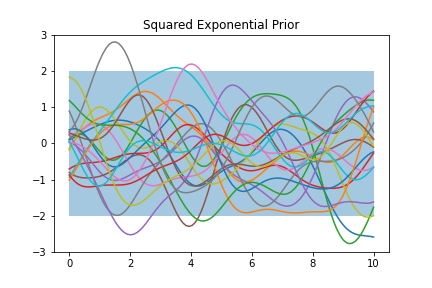
\includegraphics[width=4in]{img/05_3/gp_prior.png}
	\caption[GP prior samples]
	{Samples from a Gaussian Process prior with a squared exponential kernel. To add to the draws, the 95\% confidence interval is highlighted with a blue background. }
	\label{fig:prior_squ_exp}
\end{figure}
Then, we introduce data points, which were randomly generated using a modified sine function with added gaussian noise, see figure \ref{fig:generated_data}. 
\begin{figure}[h!]%data points to train on
	\centering
	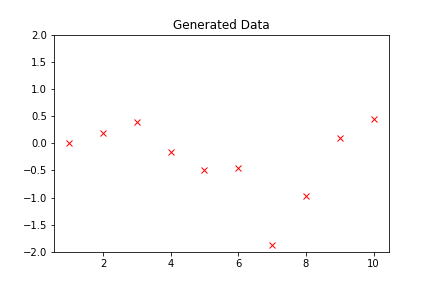
\includegraphics[width=4in]{img/05_3/generated_data.png}
	\caption[Random data from sine function with Gaussian noise]
	{Data generated from a sine function with added Gaussian noise.}
	\label{fig:generated_data}
\end{figure}
Using the learning equations \ref{eq:Key_predictive_equations_for_GP_reg}, we can train a Gaussian process on the data points and find the following posterior samples, see figure \ref{fig:GP_sqexp_samples} and confidence intervals, having solved the Gaussian Process. 
\begin{figure}[h!]
	\centering
	\begin{minipage}{0.45\textwidth}
		\centering
		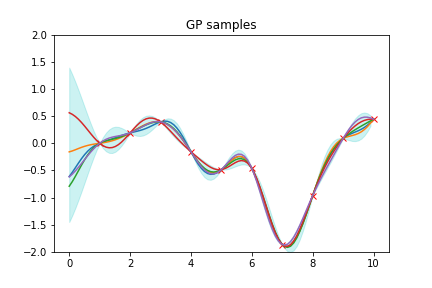
\includegraphics[scale=0.6]{img/05_3/gp_samples.png} % first figure itself
		\caption[Trained GP samples with covariance interval]{The GP conditioned on the generated dataset, with the 95\% confidence interval and 5 samples drawn from the GP. }
		\label{fig:GP_sqexp_samples}
	\end{minipage}\hfill
	\begin{minipage}{0.45\textwidth}
		\centering
		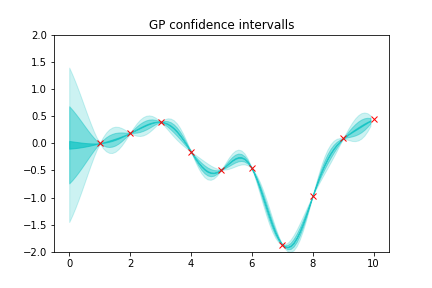
\includegraphics[scale=0.6]{img/05_3/gp_confints.png} % second figure itself
		\caption[Trained GP with covariance intervals]{The GP conditioned on the generated dataset, with confidence intervals drawn into the graph as blue shading. }
		\label{fig:GP_confidence_intervals}
	\end{minipage}
\end{figure}
The confidence intervals in figure \ref{fig:GP_confidence_intervals} have 1, 2, and 3 $\sigma$. This depiction also highlights the interpretation of GP predictions as probability distributions. \newpage
\label{sec:gp}
\cleardoubleoddpage

\subsection{Gaussian Kernel Functions}
A covariance function, or kernel function is a key part of the model used. Since not any function linking two inputs $x$ and $x'$ will in general be a viable kernel function, necessary, as well as useful properties of kernel functions need to be discussed. First, kernel functions must be positive semidefinite, 
\begin{equation}%positive semidefiniteness of kernel functions
	\int k(\bm{x},\bm{x'})f(\bm{x})f(\bm{x'})d\mu(\bm{x})d\mu(\bm{x'}) \geq 0.
\label{eq:positive_semidefiniteness_of_kernel_functions}
\end{equation}
Here, $\mu$ denotes a respective measure. Kernel functions also can be stationary, when it is a function of $\bm{x} - \bm{x'}$, exhibiting translation invariance in input space. A kernel function can be isotropic, a function of $|\bm{x} - \bm{x'}|$, making it invariant to all rigid motions. Isotropic kernel functions are also known as radial basis functions (RBF). If the kernel function is a function of $\bm{x} \cdot \bm{x'}$, it is called a dot-product kernel function. These are invariant to a rotation of coordinates about the origin, but not translation. Kernel functions also are the underlying reason for some properties concerning the total process, e.g. mean-square continuity and differentiability. \newline
\textbf{Continuity:} Continuity is a property of the Gaussian process, directly exhibited from the choice of kernel function. A stochastic process is continuous, if in a sequence of points $x_1, x_2, ..$ with another fixed point $_x*$ in $\mathbb{R}^D$ $|\bm{x}_k - \bm{x}_*| \to 0$ as $k \to \infty$. Then a process $f(x)$ is continuous in mean-square at $x_*$ if $\mathbb{E}[|f(x_k)-f(x_*)|^2] \to 0$, as $k \to \infty$. If this holds for all $x_* \in A$ where $A$ is a subset of $\mathbb{R}^D$, then $f(x)$ is said to be continuous in mean square over $A$. A random field is continuous in mean square if and only if its covariance function is continuous at $x=x_*=x'$. 
For stationary covariance funtions this reduces to checking continuity at $k(0)$. \newline
\textbf{Differentiability:} Using the mean square derivative of $f(x)$ in \textit{i}th direction 
\begin{equation}%mean square derivative of i-th direction
	\frac{\partial f(x)}{\partial x_i} = \lim_{h \to 0} \frac{f(x+h\bm{e}_i)-f(x)}{h},
\label{eq:mean_square_derivative_of_i-th_direction}
\end{equation}
and checking if the limit exists for order $2k$ and is finite at $x=0$, then the \textit{k}th order limit exists as a mean square limit. Here, the properties of the kernel around $0$ determine the smoothness properties of a stationary process. \newline \newline
Following, some of the more prominent kernel functions are presented, with some practical properties. Almost all of the following are stationary and non-degenerate, meaning they are stationary and of infinite rank.\newline
\begin{equation}%linear kernel function
	k_{linear}(\bm{x_i}, \bm{x_j}) = \sigma^2 \bm{x_i}^{\top} \cdot \bm{x_j} 
\label{eq:linear_kernel_function}
\end{equation}
is the linear kernel. As the most simple of kernels, it is as an exceptional case in this listing neither stationary, nor non-degenerate. 
\begin{equation}%exponential kernel function
	k_{exp}(\bm{x_i}, \bm{x_j}) = exp(-\frac{1}{2l}d_{ij}),
\label{eq:exponential_kernel_function}
\end{equation}
the exponential kernel, where $d_{ij} = ||\bm{x}_i - \bm{x}_j||_2$ is the Euclidian distance between the input arguments. 
\begin{equation}%squared exponential kernel
	k_{sqe}(\bm{x_i}, \bm{x_j}) = exp(-\frac{1}{2l^2}d_{ij}^2)
\label{eq:squared_exponential_kernel}
\end{equation}
is the squared exponential kernel. It is also known as radial basis function. 
\begin{equation}%matern 32 kernel
	k_{mat32}(\bm{x_i}, \bm{x_j}) = \Bigg( 1 + \frac{\sqrt{3}d_{ij}}{l} \Bigg) exp \Bigg( - \frac{\sqrt{3}}{2l} d_{ij} \Bigg)
\label{eq:matern_32_kernel}
\end{equation}
is the Matern3/2 kernel. it is a special case like the Matern5/2 kernel
\begin{equation}%matern 52 kernel
	k_{mat52} = \Bigg( 1+ \frac{\sqrt{5}d_{ij}}{l} + \frac{5r^2}{3l^2} \Bigg)exp\Bigg( \frac{\sqrt{5}d_{ij}}{l} \Bigg)
\label{eq:matern_52_kernel}
\end{equation}
of the Matern class of kernels
\begin{equation}%matern kernel class
	k_{mat} = \frac{2^{1-\nu}}{\Gamma(\nu)} \Big( \frac{\sqrt{2\nu}d_{ij}}{l} \Big)^\nu K_\nu \Big( \frac{\sqrt{2 \nu}d_{ij}}{l} \Big) .
\label{eq:matern_kernel_class}
\end{equation}
The matern kernels can be constructed with positive parameter $\nu$, $K_\nu$ is a modified Bessel function. Also, as $\nu \to \infty$ the function becomes the smooth squared exponential kernel, for $\nu = 1/2$ the Matern class kernel becomes the Ornstein-Uhlenbeck kernel. This kernel gives rise to a continuous-time AR(p) Gaussian process. But since this kernel was not used in the further work, it will not be discussed more. Kernel functions are used to calculate the entries of the covariance matrices. Different kernel functions apply better or worse to different problems. Even though there sometimes are kernel function choices that seem more applicable to a problem from prior assumptions, different kernel functions should be used and compared to ensure better models. 
\newline \newline
On another note, novel kernels can be created through different methods, for example by combining different existing kernels. Since kernels are always independent, kernels can be added to create a new kernel. For the same reason the multiplication of two kernels also produces a new kernel. In addition, new kernels can be created using rescaling, where kernels are e.g. normalized, or through convolution, where the kernels are mapped onto other spaces. Another major part of the properties of kernel functions are hyperparameters. These influence for example the frequency of changes exhibited by a kernel function. This hyperparameter, usually denoted as $l$ is often called kernel lengthscale. An example, of how this parameter influences the model is shown in figure \ref{fig:lengthscale}.
\begin{figure}%lengthscale
	\label{fig:lengthscale}
	\centering
	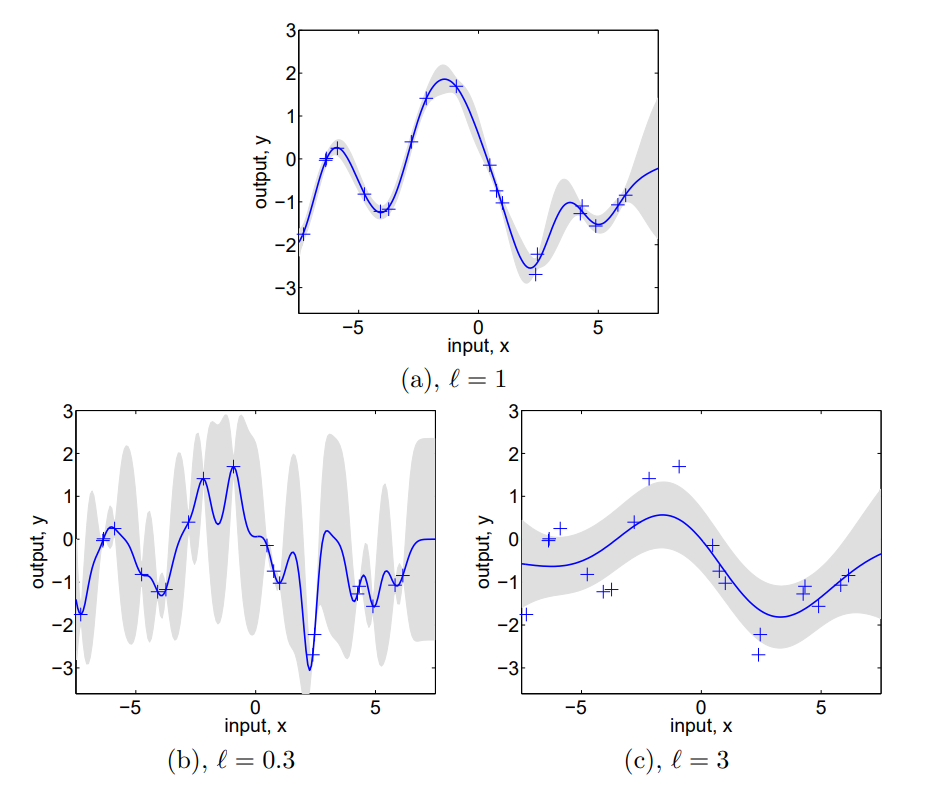
\includegraphics[width=4in]{img/05_4/lengthscale.png}
	\caption[Lengthscale influence on samples]
	{Comparison of hyperparameters for the squared exponential kernel function. A large lengthscale exhibits properties where the function does not react to changes quickly, while a small lengthscale gives the opportunity to react to changes almost immediately. While small lengthscales usually lead to better fits, the prediction power often decreases since more information from noise is incorporated into the covariance matrix. The data is generated from a GP with $l_a=0.3$, $l_b=1$, $l_c=3$, $\sigma_f=1$, and $\sigma_n=0.1$ \cite{Rasmussen_06}. The panel a has lengthscale $l_a$, panel b has lengthscale $l_b$, and panel c $l_c$.}
\end{figure}
The variances, often denoted by $\sigma_n$ for the noise variance, and $\sigma_f$ for the kernel function variance, influence the confidence interval in which we assume the functions to lie. $\sigma_n$ stems from the noise we attribute to the special systemic noise of the problem at hand, while $\sigma_f$ stems from just observing data that is noisy. A large noise variance and kernel variance will exhibit the kernel matrix incorporating a larger error tolerance. This can be seen in the enlargening of the confidence intervals on the draws of functions from the same process. Higher Variances lead to more flexible fitting, while lower variances will be more rigid. On the other hand, if variances are too high or too low, essential information about the structure of the problem can get lost.
\label{sec:kernels}
\cleardoubleoddpage

\section{Gaussian Process Latent Variable Models}
Latent variables are variables of an experiment or theory, that influence the outcome of an experiment without being directly measurable. The only way to obtain a latent variable is to infer it from the information that can be observed in the experiment. Intelligence, for example, is a latent variable. It is not directly measurable, but is influencing the outcome of some experiments in psychology. While tests for intelligence try to measure intelligence by inferring it, they can only give a general direction of the true value, assuming it exists and can be ascertained to a single value in a controlled environment. The test then tries to measure what we believe to be components of intelligence, e.g. skills in logic, pattern recognition and grammar. The measured scores are then used to calculate an overall score, which we believe to be a measure for intelligence. While latent variable models, such as the one used in psychology to infer intelligence from a test, enable scientists to more accurately describe phenomena we already have a general understanding about, the models also enable us to infer data in other fields. Since latent variable models are already directly connected to statistics, it is not a far stretch to apply some of them in fields that previously used almost exclusively statistical methods to describe phenomena. Also, latent variable models could reveal relations between different variables of the system, if different variables are dependent on the same set of latent variables, and therefore change with a behaviour that can be infered by knowing the state of the latent variables. \newline
Assume that a data matrix $Y \in \mathbb{R}^{N\times D}$ is given and the goal is to find a lower dimensional representation $X \in \mathbb{R}^{N\times Q}$ of the matrix, without loosing a major share of the information encoded in the data matrix. Previous models have mostly used Principal Component Analysis (PCA) to achieve this dimensionality reduction. Principal Component Analysis has also been shown to be the maximum likelihood solution to a particular form of Gaussian Latent Variable Model \cite{Tipping_Bishop_1999_1}\cite{Tipping_Bishop_1999_2}. PCA here embeds $\mathcal{Y}$, the data space, via linear mapping into a latent space $\mathcal{X}$. Later on, the Gaussian Process Latent Variable Model was introduced as a non-linear extension to probabilistic PCA \cite{Lawrence_2005}. \newline \newline
Probabilistic PCA (P-PCA) is a model derived by using the probabilistic framework. While P-PCA facilitates statistical testing and Bayesian workflows, it can also be applied to problem sets, where PCA previously could not be used efficiently. This is especially the case for missing data in the dataset. Also, P-PCA can be represented as a general Gaussian density model, which can efficiently be solved through computing maximum likelihood estimates for the parameters associated with the covariance matrix from principal components. This promises effective classification and novelty detection. Starting with factor analysis, a linear relation between the observation vector $\bm{t} \in \mathbb{R}^d$ and the vector of latent variables $\bm{x} \in \mathbb{R}^q \text{, } d>q$ can be established like 
\begin{equation}%Factor analysis
	\bm{t} = W\bm{x} + \bm{\mu} + \bm{\epsilon}
\label{eq:Factor_Analysis}
\end{equation}
with noise $\bm{\epsilon} \sim \mathcal{N}(\bm{0, \Sigma})$ and mean vector $\bm{\mu}$ to permit the model with a non-zero mean. It promises a parsimonious explanation of dependencies between observations. If $\bm{x}$ is assumed to be standard Gaussian, we can find the distribution for $t$ 
\begin{equation}%factor analysis results
	\bm{t} \sim \mathcal{N}(\bm{\mu}, WW^{\top} + \Sigma).
\label{eq: Factor analysis results}
\end{equation}
Now, when constraining the covariance matrix $\Sigma$ to be a diagonal matrix, we will have only autocorrelation in observed variables (conditional independence), given the latent variables $\bm{x}$ and the mapping $W$. The latent variables are therefore used to explain correlations between observation variables. \newline
With this, we can find P-PCA by considering the $\bm{x}$-conditional probability distribution over $\bm{t}$-space
\begin{equation}%x-conditional probability dist over t-space
	\bm{t}|\bm{x} \sim \mathcal{N}(W\bm{x} + \bm{\mu}, \sigma^2I)
\label{eq: x-conditional probability dist over t-space}
\end{equation}
Integrating out the latent variables, we arrive at the Gaussian marginal distribution for $\bm{t}$
\begin{equation}%marginal distribution t
	\bm{t} \sim \mathcal{N}(\bm{\mu}, WW^{\top} + \sigma^2I)
\label{eq: marginal distribution t}
\end{equation}
with corresponding log-likelihood
\begin{equation}%log likelihood p-pca
	\log p(\bm{t}) = -\frac{N}{2} \Big(d \ln(2\pi) + \ln|WW^{\top} + \sigma^2I| + \text{tr}((WW^{\top} + \sigma^2I)^{-1}\frac{1}{N}\sum_{n=1}^{N}(\bm{t}_n - \bm{\mu})(\bm{t}_n - \bm{\mu})^{\top}) \Big).
\label{eq: log likelihood p-pca}
\end{equation}
Iterative maximisation of the log-likelihood now presents a fast and reliable way to optimise the P-PCA. From this model, standard PCA can be recovered when $\sigma^2 \to 0$ and $ WW^{\top} + \sigma^2I \to (W_{ML}^{\top}W_{ML})$. 
\newline \newline
Considering the GPLVM, we can find the generating procedure to be
\begin{equation}%generating procedure GPLVM
	Y_{n,:} = \bm{f}(X_{n,:}) + \bm{\epsilon}_n,
\label{eq: generating procedure GPLVM}
\end{equation} 
closely resembling the linear model of a GP, equation \ref{eq:Factor_Analysis} again. Here, $\bm{f} = f(f_1,...,f_D)$ is a group of $D$ independent samples from a Gaussian process $f_d \sim \mathcal{GP}(0, k(\cdot,\cdot))$. $X$ is the matrix containing the latent space ($\mathcal{X}$) positions.  Due to the structure of the problem at hand, the rows of the data matrix $Y$ are assumed to be jointly Gaussian distributed, while the columns are independent. This can be interpreted as every data point (return rate) of a single day being Gaussian distributed, while there is no time-dynamic. Each sample of $Y_{:,d} \sim \mathcal{N}(Y_{:,d}|\bm{0}, K)$ is assumed to incorporate noise inside the covariance matrix $K = k(X,X) + \sigma^2 I$, where $\sigma^2$ is the variance of the noise $\bm{\epsilon}$, which is assumed to be random. We find the marginal likelihood of $Y$ to be
\begin{equation}%marginal likelihood of data gplvm
	p(Y|X) = \prod_{d=1}^{D} \mathcal{N}(Y_{:,d}|\bm{0},K) = \frac{1}{(2\pi)^{ND/2}|K|^{D/2}} \exp \Bigg(-\frac{1}{2}tr(K^{-1}YY^{\top})\Bigg).
\label{eq: marginal likelihood of data gplvm}
\end{equation}
The covariance matrix $K$ gives the dependency on the kernel hyperparameters as well as the latent space positions $X$. Lawrence (2005) suggested to optimize the log-marginal-likelihood $\log p(Y|X)$, with the hyperparameters and latent space positions as the parameters used for optimisation. 
\label{sec:GPLVM}
\cleardoubleoddpage

\subsection{Student-t-Process}
An alternative to the Gaussian processes provide the Student-t-processes \cite{Shah_14}. They can be regarded as a generalized Gaussian process. Assuming an inverse Wishart prior for the kernel of a Gaussian process will result in a Student-t process. Due to this, we can also think of the Student-t process as a prior over functions, that is non-parametric. Also belonging to the family of elliptical processes, the Student-t process ($\mathcal{TP}$) offers more robustness to outliers inherent to the process, due to the broader flanks of the Student-t distribution. It is the most general elliptically symmetric process for which analytical marginal and predictive distributions exist. While some argue \cite{Shah_14}, that the predictive covariances of a Gaussian process do not depend on the training observations, the predictive covariances from a Student-t process do depend on training observations. Deriving the Student-t process, we will start with a Wishart process $W_n(\nu,K)$. The Wishart distribution is a distribution over the set of real-valued symmetric matrices, of size $n\times n$, that are positive definite $\Pi(n)$. The density function is
\begin{subequations}%Wishart distribution
	\label{eq:}
	\begin{align}
	\Sigma \sim W_n(\nu,K) \text{, if }         \label{eq:Wishart Distribution} \\
	p(\Sigma) = \Big(|K|^{\nu/2}2^{\nu n/2} \Gamma_n(\nu/2)\Big)^{-1}|\Sigma|^{(\nu-n-1)/2} exp \Big(-\frac{1}{2}tr(K^{-1}\Sigma)\Big)         \label{eq:Wishart distribution definition}
	\end{align}
\end{subequations}
with $\nu > n-1,\text{ } \nu \in \mathbb{R}_+$. This definition exhibits the marginalisation property, just like a GP. But since for $\nu \to \infty$ almost surely $\nu^{-1}\Sigma \to K$, thereby loosing the usefulness of the process. This property is not exhibited in the inverse Wishart process ($Iw_n(\nu, K)$) \cite{Dawid_1981}.
\begin{subequations}%Inverse Wishart Distribution
	\label{eq:}
	\begin{align}
	\Sigma \sim IW_n(\nu,K) \text{ if }         \label{eq:Inverse Wishart distribution} \\
	p(\Sigma) = \Big(\frac{|K|^{(\nu+n-1)/2}}{2^{(\nu+n-1)n/2}\Gamma_n((\nu+n-1)/2)}\Big)^{-1}|\Sigma|^{-(\nu+n-1)/2} exp \Big(-\frac{1}{2}tr(K\Sigma^{-1})\Big)         \label{eq:Inverse Wishart distribution definition}
	\end{align}
\end{subequations}
This formulation requires $\nu > 2$ and $\mathbb{E}[\Sigma] = (\nu-2)^{-1}K$, for the mean and the covariance to exist. Both Wishart distributions place prior mass on every possible matrix $\Sigma$ stemming from the set $\Pi(n)$. It was also previously shown, that the Inverse Wishart distribution is consistent under marginalization. Any submatrix $\Sigma_{11}$ will be $Iw_{n1}(\nu_1K-\Sigma_{11})$ distributed. With this, we can define a Inverse Wishart Process analogous to a Gaussian process with a base kernel $k:\mathcal{X} \times \mathcal{X}\to \mathbb{R}$
\begin{equation}%Inverse Wishart Process
	\sigma \sim \mathcal{IWP}(\nu,k(\cdot,\cdot)).
\label{eq: Inverse Wishart Process}
\end{equation}
If the Inverse Wishart process is applied as prior on the kernel function of a $\mathcal{GP}$, a Student-t process 
\begin{subequations}%Student-t process
	\label{eq:Student-t process}
	\begin{align}
	\sigma \sim \mathcal{IWP}(\nu,k_\theta)         \label{eq:inverse wishart covariance kernel} \\
	\bm{y}|\sigma \sim \mathcal{GP}(\mu, (\nu-2)\sigma)         \label{eq:hierarchical gaussian process with iwp kernel}
	\end{align}
\end{subequations}
generative approach is achieved. We find the data to be Student-t distributed if the density is of the structure
\begin{subequations}%student-t distributed data
	\label{eq:multivariate Student-t distributed data}
	\begin{align}
	\bm{y} \sim \mathcal{MVT}_n(\nu,\bm{\mu},K)         \label{eq:multivariate Student-t shorthand} \\
	p(\bm{y}) = \frac{\Gamma(\frac{\nu+n}{2})}{((\nu-2)\pi)^{\pi/2}\Gamma(\nu/2)}|K|^{-1/2}\Big(1+\frac{(\bm{y}-\bm{\mu})^{\top}K^{-1}(\bm{y}-\bm{\mu})}{\nu-2}\Big)^{-(\nu+n)/2} ,        \label{eq:multivariate Student-t distributed data def}
	\end{align}
\end{subequations}
for which the mean and covariance are given by
\begin{subequations}%mean and cov studt
	\label{eq:mean and cov studt}
	\begin{align}
	\mathbb{E}[\bm{y}] = \mathbb{E}[\mathbb{E}[\bm{y}|\Sigma]] = \bm{\mu}         \label{eq:mean studt} \\
	cov[\bm{y}] = \mathbb{E}[\mathbb{E}[(\bm{y}-\bm{\mu})(\bm{y}-\bm{\mu})^{\top}|\Sigma]]         \label{eq:cov studt}
	\end{align}
\end{subequations}
\cite{Shah_14}. The Student-t process is consistent under marginalisation. As a shorthand, we write $f \sim \mathcal{TP}(\nu, \bm{\mu},K)$ for a joint Student-t process over a finite collection of function values, as a similar counterpart to the Gaussian process over function values \ref{eq:Gaussian_process_function_space_view}. The student-t process generalizes the Gaussian process through the introduction of the degree of freedom parameter $\nu$. For  $\nu \to \infty$ we arrive at a Gaussian process, while at $\nu = 1$ we have a Cauchy process. Analyzing this hyperparameter, we find that it controls how much probability mass lies in the tails of a distribution, directly influencing how large of a variance samples from a Student-t process have compared to a Gaussian process.
\begin{figure}[h!]%Comparison GP and TP samples
	\centering
	\begin{minipage}{0.75\textwidth}
		\centering
		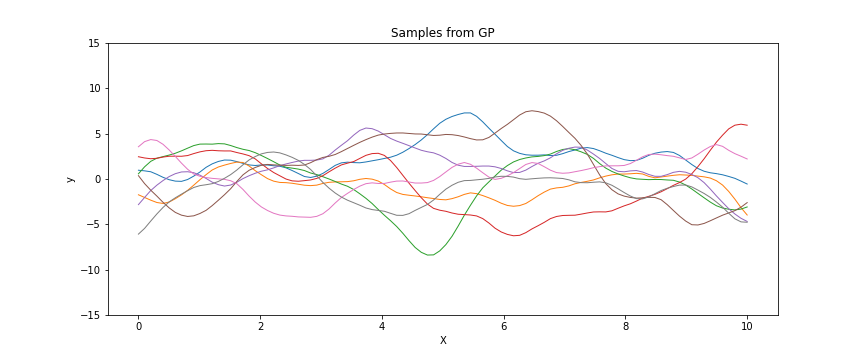
\includegraphics[scale=0.4]{img/05_8/GP_samples.png} % first figure itself
		\caption[GP samples example]{Samples from a GP.}
		\label{fig:GP_samples}
	\end{minipage}\hfill
	\begin{minipage}{0.75\textwidth}
		\centering
		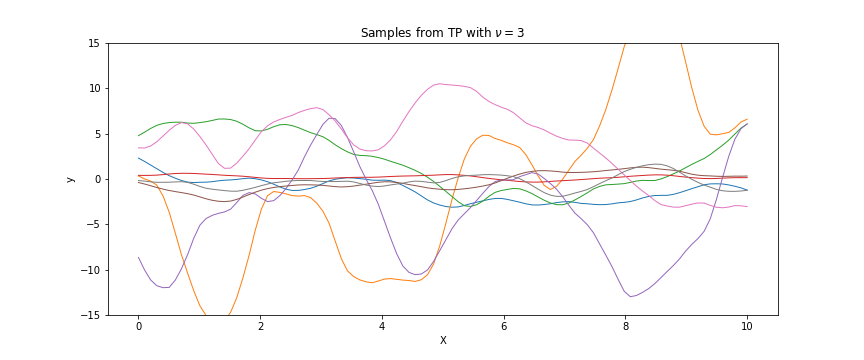
\includegraphics[scale=0.4]{img/05_8/TP_samples.png} % second figure itself
		\caption[TP samples example]{Samples from a TP.}
		\label{fig:TP_samples}
	\end{minipage}
\end{figure}
In figures \ref{fig:GP_samples} and \ref{fig:TP_samples}, the comparison of Gaussian process prior samples (upper) and Student-t (lower) process prior samples are shown. In general the Student-t samples have a broader credibility predictive sample interval compared to the Gaussian process. This leads to a higher tolerance for outliers in the data sets, since the outliers do not impact the covariance as much as with a Gaussian process. A higher parameter $\nu$ leads to a more narrow credibility interval.
After analysing the properties of a Student-t process prior, the conditional distributions can be analyzed. Splitting up a data set into e.g. a test ($\bm{y}_*$) and training ($\bm{y}$) dataset, the respective multivariate Student-t process becomes
\begin{subequations}%multivariate student t conditional distribution
	\label{eq:multivariate student t conditional distribution}
	\begin{align}
	\scriptstyle
	\bm{y}_*|\bm{y} \sim \mathcal{MVT}_{n_*}(\nu+n, K(X_*,X)K(X,X)^{-1}(\bm{y}-\bm{\mu})+\bm{\mu_*},  \nonumber \\
	\scriptstyle
	 \frac{\nu+(\bm{y}-\bm{\mu})^{\top}K(X,X)^{-1}(\bm{y}-\bm{\mu})-2 }{\nu+n-2}(K(X_*,X_*)-K(X_*,X)K(X,X)^{-1}K(X,X_*))) 
	\end{align}
\end{subequations}
with number of datapoints $n_*$ in $\bm{y}_*$ and $n$ in $\bm{y}$ respectively. 
\label{sec:student-t}
\cleardoubleoddpage


\section{Algorithms for stochastic problem computation}
Markov Chain Monte Carlo (MCMC) methods \cite{Geyer_2011} are a class of algorithms that are used to sample a probability distribution that is analytically intractable, or just very complex. A Markov Chain is constructed, that has the same distribution as the target distribution, and recording the chain, the target distribution is uncovered. Since MCMC methods only uncover the true target distribution for very large chain lengths, or even infinite length, a practical convergence criterion is needed to numerically approximate the target multidimensional distributions. We know, that target distributions are calculated via solving integrals of the form \ref{eq:Bayes_with_intractable_term}, so MCMC methods are a likely choice to base further evaluations on. An example of this is depicted in the following figure, where an algorithm is shown that lets the test distribution converge towards the target distribution using the metropolis hastings algorithm.
\begin{figure}[h!]%Metropolis Hastings Convergence Example
	\centering
	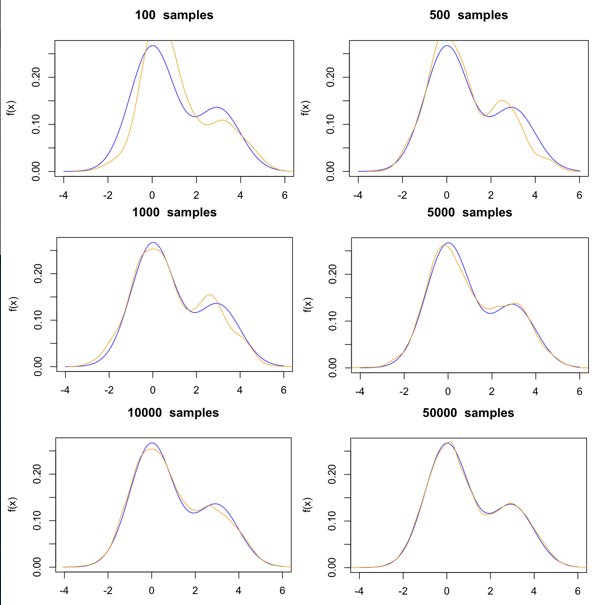
\includegraphics[width=4in]{img/05_6/MetropolisHastingsConvergence.png}
	\caption[Metropolis Hastings Convergence Example]
	{Convergence of the Metropolis Hastings algorithm as an example for Markov chain Monte Carlo methods approximating the target distribution of a bayesian problem. It is clear that more samples lead to a better approximation of the target distribution.}
\end{figure}
A necessary precondition is that the probability density of the target random variable is given up to a constant. If the integral is intractable, MCMC methods can evaluate the integral statistically by generating an ensemble of chains starting at arbitrarily chosen points. A chain is a stochastic process, that moves around randomly on this high dimensional probability surface where moves are generated via Monte Carlo sampling, and then an evaluation of the contribution of this place to the integral is carried out. If the posterior mass is low in some regions, the chain will move away faster from this location, while on the other hand it will spend more moves in regions with higher posterior mass. These Markov chains then have an equilibrium distribution proportional to the target distribution. MCMC methods, even though outperforming generic Monte Carlo algorithms, still suffer from the curse of dimensionality, where regions of higher probability tend to stretch due to a high number of dimensions. Regions with higher probability mass then do not get the proportion of moves necessary in the faster scaling volume of high dimensional space, and contribute less to the solution. This method also implies a problem of when to accept a chain to be converged to a stationary distribution with a reasonable error. Here, the term of rapid mixing becomes important, describing the phenomenon of stationary distributions being reached quickly while starting from arbitrary positions, highlighting the need to sample several chains for non-variational inference algorithms. An extension of the central limit theorem, the Markov chain central limit theorem \cite{Andrieu_2003}, states that for a sequence of random elements forming a Markov chain with the Markov property, the mean of the Markov chain will tend towards a normal distribution. Formally, we have a sequence of random elements $X_1, X_2, X_3, ...$ of some set $\mathcal{X}$ forming the Markov chain with a stationary probability distribution. Also, the initial distribution of the process, the distribution leading to $X_1$ has to be stationary, which entails that $X_1, X_2, X_3, ...$ are identically distributed. Then, the Markov property is necessary, and we need a measurable real-valued function $g$ with $var(g(X_1))<+\infty$.
\begin{subequations}%markov chain central limit theorem prerequisites
	\label{eq:markov chain central limit theorem prerequisites}
	\begin{align}
	\mu = \mathbb{E}(g(X_1)),                                                    \label{eq:mean of initial markov chain step} \\
	\sigma^2 = var(g(X_1)) + 2\sum_{k=1}^{\infty}cov(g(X_1), g(X_{1+k})),         \label{eq:variance markov steps} \\
	\hat{\mu}_n = \frac{1}{n} \sum_{k=1}^{n}g(X_k).                               \label{eq:expected mean markov process}
	\end{align}
\end{subequations}
For $n \to \infty$, we find:
\begin{equation}%markov chain convergence
	\label{eq:markov chain convergence}
	\sqrt{n}(\hat{\mu_n}-\mu) \to \mathcal{N}(0, \sigma^2),         
\end{equation}
resulting in an important feature for convergence. Furthermore, a solution to the curse of dimensionality would be to accept higher autocorrelation and expensive computations by using smaller steps of the chain, which is impractical. More sophisticated methods, like Hamiltonian Monte Carlo reduce autocorrelation while keeping the chain in the desired regions of the probability surface. 

\subsubsection{Hamiltonian Monte Carlo}
Hamiltonian Monte Carlo (HMC) \cite{Duane_1987} is a MCMC method that applies derivatives of the density function to generate efficient transitions when approximating the posterior. The dynamics of the chain is given by Hamiltons equations of motion. The Hamiltonian dynamics simulation is carried out using numerical integration. To achieve this, HMC uses auxiliary momentum variables to form a joint density to draw from. 
\begin{equation}%HMC joint density for regular and auxiliar variables
	p(\rho, \theta) = p(\rho | \theta) p(\theta),
\label{eq: HMC joint density for regular and auxiliar variables}
\end{equation}
where $\rho$ are the auxiliary momentan variables, and $\theta$ are the parameters of the model. By choosing the following distribution for $\rho$, it becomes independent of $\theta$.
\begin{equation}%HMC independent auxiliary variables
	\rho \thicksim \mathcal{N}(0,M).
\label{eq:HMC_independent_auxiliary_variables}
\end{equation}
Here, $M$ is the Euclidian metric, which is just a transformation of parameter space to enhance the efficiency of sampling. The joint density of auxiliary and regular parameters then leads to the combined Hamiltonian
\begin{equation}%HMC Hamiltonian
	H(\rho,\theta) = -log(p(\rho, \theta)) = -log(p(\rho | \theta)) - log(p(\theta)) = T(\rho | \theta) + V(\theta),
\label{eq: HMC Hamiltonian}
\end{equation}
where we define $T(\rho | \theta)$ and $V(\theta)$ as kinetic energy and potential energy respectively, directly analogous to physics. in statistics we find that $T(\rho | \theta) = -log(p(\rho | \theta))$ and $V(\theta) = log(p(\theta))$. The potential energy is often in a statistical context regarded as a log density. From this on, we can use Hamilton´s equations to find find the momentum needed for state transitions. The momentum parameter values are independently drawn using \ref{eq:HMC_independent_auxiliary_variables}, so that momentum is changing across iterations. We use
\begin{subequations}%HMC Hamiltonian equations
	\label{eq:HMC Hamiltonian equations}
	\begin{align}
	\frac{d\theta}{dt} = \frac{\partial H}{\partial \rho} = \frac{\partial T}{\partial \rho},         \label{eq:HMC parameter Hamilton equation} \\
	\frac{d\rho}{dt} = -\frac{\partial H}{\partial \theta} = \frac{\partial T}{\partial \theta} - \frac{\partial V}{\partial \theta} = - \frac{\partial V}{\partial \theta},         \label{eq:HMC auxiliary Hamiltonian equation}
	\end{align}
\end{subequations}
where we have recognized the momentum density $\partial T/\partial \theta$ to be zero, due to the independence of momentum density and target density. This two-state differential equation can then be solved using many integrators. We will discuss the Leapfrog integrator here, since it is most widely used in HMC implementations. In general the Leapfrog integrator uses half integer time steps to calculate velocities and integer time steps to calculate  positions, which pans out to the following updating equations:
\begin{subequations}%HMC Leapfrog update equations
	\label{eq:HMC Leapfrog update equations}
	\begin{align}
	\rho \leftarrow \rho - \frac{\epsilon}{2}\frac{\partial V}{\partial \theta},         \label{eq:LF update rule momentum} \\
	\theta \leftarrow \theta + \epsilon M^{-1}\rho.         \label{eq:LF update rule pamaeters}  
	\end{align}
\end{subequations}
Here, the first update rule is carried out twice, once at the start of a timestep and once at the end. The symplectic Leapfrog integrator has a $\mathcal{O}(\epsilon^3)$ error per step, and globally an error of $\mathcal{O}(\epsilon^2)$. Following a calculated transition, the Metropolis acceptance step begins, where evaluation of the energy of the Hamiltonian leads to accepting the proposed step, or throwing this set of parameters away. The probability of keeping a step can be calculated via
\begin{equation}%Metropolis Acceptance probability of a HMC step
	min(1, exp(H(\rho, \theta))-exp(H(\rho^*, \theta^*))),
\label{eq: Metropolis Acceptance probability of a HMC step.}
\end{equation}
where $\rho^*, \theta^*$ are the proposed values and $\rho, \theta$ the origin of the proposed transition. We do not have to implement HMC by ourself. We can use probabilistic programming languages such as stan. For that, we onl yghave to define the unnormalized posterior density and the approximation thereof is carried out by stan.

\subsubsection{Stochastic Gradient Ascent}
\label{sec:stochastic_gradient_ascent}
Stans variational inference algorithm, Automatic Differentiation Variational Inference \cite{Kucukelbir_2015}, optimizes the ELBO in real-coordinate space. The stochastic gradient ascent obtains unbiased, yet noisy gradients through automatic differentiation and evaluates the ELBO using Monte Carlo integration. Along these gradients, the algorithm ascends using a sequence of adaptive stepsizes. Typically, in practice, the ELBO is sampled with around 100 samples, so that the true ELBO value can be approximated with reasonably high confidence. The ELBO is only evaluated every few iterations, to save computation time, but inside high dimensional manifolds, this seems not to be a problem in practice \cite{stan_manual}. The gradients are also approximated using Monte Carlo Integration, but usually only one sample is drawn, as experience has shown that, while remaining high computational efficiency, stochastic gradient ascent is capable of following such gradients nonetheless. Adaptive step sizes are optimized during a warmup phase where a good value for the single exposed parameter is selected from values spanning multiple orders of magnitude \cite{stan_manual}. This parameter is then used in combination with a finite memory version of adaGrad \cite{Duchi_2011}. In the end, every calculation needs to asses convergence, but since there are no closed form analytical expressions available, the progression of the ELBO values has to be tracked. Using a rolling window, which is heuristically determined, in which the average and median change of the ELBO are computed, we assume convergence if either of those values has fallen below a certain threshold. 
\label{sec:mcmc}
\cleardoubleoddpage
